\subsection{Track Coasting Correct}
\label{sec:eval_req_trk_coast_correct} 

\subsubsection{Configuration}

\begin{figure}[H]
    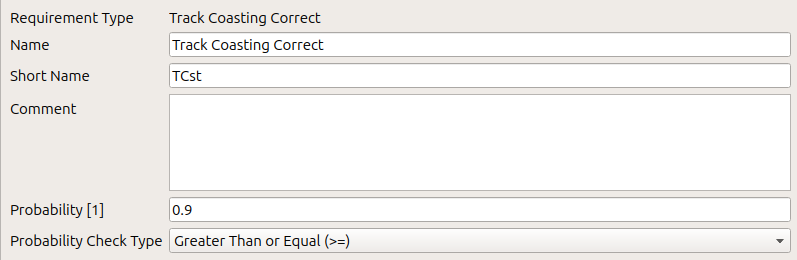
\includegraphics[width=14cm,frame]{figures/eval_req_coasting.png}
  \caption{Evaluation Track Coasting Correct Requirement}
\end{figure}

The 'Track Coasting Correct’ requirement is used to calculate the probability of a target report having a difference in the track coasting flag. 

\begin{itemize}  
\item Probability [1]: Probability of correct coasting flag
\item Probability Check Type: $\geq$
\end{itemize}
\ \\

\subsubsection{Calculation}

The track coasting flag of the test data is compared to the two reference updates closest in time (before and after the test timestamp), if one of the reference flag values matches, the target report is counted for the calculated probability PCCoast (probability of correct track coasting). The PCCoast must in turn pass the check for the requirement to pass. 

\subsubsection{Result Values}

\paragraph{Sector}

\begin{center}
 \begin{table}[H]
  \begin{tabularx}{\textwidth}{ | l | X |  l | }
    \hline
    \textbf{Name} & \textbf{Description} & \textbf{Example} \\ \hline
    Sector Layer & Name of the sector layer & units\_OPS\_2024 \\ \hline
    Requirement Group & Name of the requirement group & Mandatory \\ \hline
    Requirement & Name of the requirement & Track Coasting Correct \\ \hline
    Num Results & Total number of results & 1502 \\ \hline
    Num Usable Results & Number of usable results & 1500 \\ \hline
    Num Unusable Results & Number of unusable results & 2 \\ \hline
    Use & To be used in results & true \\ \hline
    \#Up [1] & Number of updates & 583571 \\ \hline
    \#NoRef [1] & Number of updates w/o reference position or Track Coasting & 0 \\ \hline
    \#NoRefPos [1] & Number of updates w/o reference position & 0 \\ \hline
    \#NoRef [1] & Number of updates w/o reference Track Coasting & 0 \\ \hline
    \#PosInside [1] & Number of updates inside sector & 583277 \\ \hline
    \#PosOutside [1] & Number of updates outside sector & 294 \\ \hline
    \#Unknown [1] & Number of updates unknown Track Coasting & 0 \\ \hline
    \#Correct [1] & Number of updates with correct Track Coasting & 583248 \\ \hline
    \#False [1] & Number of updates with incorrect Track Coasting & 29 \\ \hline
    PCCoast [\%] & Probability of Correct Track Coasting & 100.00 \\ \hline
    Condition &  & >= 90.00 \\ \hline
    Condition Fulfilled &  & Passed \\ \hline
    \end{tabularx}
\end{table}
\end{center}

Also, a table is given for all single targets, sorted by PCCoast.

\paragraph{Single Target}

\begin{center}
 \begin{table}[H]
  \begin{tabularx}{\textwidth}{ | l | X |  l | }
    \hline
    \textbf{Name} & \textbf{Description} & \textbf{Example} \\ \hline
  Use & To be used in results & true \\ \hline
  \#Up [1] & Number of updates & 95 \\ \hline
  \#NoRef [1] & Number of updates w/o reference position or Track Coasting & 0 \\ \hline
  \#NoRefPos [1] & Number of updates w/o reference position  & 0 \\ \hline
  \#NoRef [1] & Number of updates w/o reference Track Coasting & 0 \\ \hline
  \#PosInside [1] & Number of updates inside sector & 95 \\ \hline
  \#PosOutside [1] & Number of updates outside sector & 0 \\ \hline
  \#Unknown [1] & Number of updates unknown Track Coasting & 0 \\ \hline
  \#Correct [1] & Number of updates with correct Track Coasting & 95 \\ \hline
  \#False [1] & Number of updates with incorrect Track Coasting & 0 \\ \hline
  PCCoast [\%] & Probability of Correct Track Coasting & 100.00 \\ \hline
  Condition &  & >= 90.00 \\ \hline
  Condition Fulfilled &  & Passed \\ \hline
\end{tabularx}
\end{table}
\end{center}
